\باب{یک سمتی رو مشین}
\اصطلاح{یک سمتی رو مشین}\فرہنگ{یک سمتی رو!مشین} یا تو یک سمتی رو\حاشیہب{dc, direct current} برقی طاقت پیدا کرتے ہیں یا پھر یہ یک سمتی رو برقی طاقت سے چلتے ہیں۔یک سمتی رو موٹروں کی اہمیت بتدریج کم ہوتی جا رہی ہے اور ان کی جگہ امالی موٹر استعمال ہونے لگے ہیں جو جدید طرز کے \اصطلاح{قوی الیکٹرانکس}\فرہنگ{قوی الیکٹرانکس}\حاشیہب{power electronics} سے قابو کئے جاتے ہیں۔موجودہ دور میں گاڑیوں میں لگے یک سمتی جنریٹر بھی دراصل سادہ بدلتی رو جنریٹر ہوتے ہیں جن کے اندر نسب \اصطلاح{ڈایوڈ}\حاشیہب{diode} ان کی بدلتی محرک برقی دباؤ کو یک سمتی محرک برقی دباؤ میں تبدیل کر دیتی ہے۔

اس باب میں دو قطب کے یک سمتی آلوں کا مطالعہ کیا جائے گا۔میکانی سمت کار رکھنے والے یک سمتی آلوں میں میدانی لچھا ساکن ہوتا ہے جبکہ قوی لچھا گھومتا ہے۔

\حصہ{میکانی سمت کار کی بنیادی کارکردگی}
جنریٹر بنیادی طور پر بدلتی رو برقی دباؤ ہی پیدا کرتا ہے۔ یک سمتی جنریٹر کے اندر نسب  \اصطلاح{سمت کار}\فرہنگ{سمت کار}\فرہنگ{commutator}\حاشیہب{commutator} میکانی طریقہ سے اس بدلتی رو کو یک سمتی رو میں تبدیل کرتا ہے اور یوں جنریٹر کی برقی سروں سے یک سمتی برقی دباؤ حاصل ہوتا ہے۔

سمت کار کو شکل \حوالہ{شکل_یکسمتی_میکانی_سمتکار}  میں دکھایا گیا ہے۔ اس شکل میں جنریٹر کے قوی  لچھے کو ایک چکر کا دکھایا گیا ہے اگرچہ حقیقت میں ایسا نہیں ہوتا۔قوی لچھے کے برقی سروں کو د اور ڈ سے ظاہر کیا گیا ہے جو سمت کار کے د اور ڈ حصوں کے ساتھ جُڑے ہیں۔قوی لچھا اور سمت کار ایک ہی دھرے پر نسب ہوتے ہیں اور یوں یہ ایک ساتھ حرکت کرتے ہیں۔تصور کریں کہ یہ دونوں گھڑی کی اُلٹی سمت مقناطیسی میدان میں گھوم رہے ہیں۔مقناطیسی میدان  اُفقی سطح میں \عددیء{N} سے \عددیء{S} کی جانب ہے جسے نوکدار لکیروں سے دکھایا گیا ہے۔ سمت کار کے ساتھ کاربن کے ساکن بُش، اسپرنگ کی مدد سے دبا کر رکھے جاتے ہیں۔ان کاربن کے بُشوں سے برقی دباؤ بیرونِ جنریٹر موصل برقی تاروں کے ذریعہ منتقل کی جاتی ہے۔ان بُشوں کو مثبت نشان یعنی \عددیء{+}  اور منفی نشان یعنی \عددیء{-} سے ظاہر کیا گیا ہے۔
\begin{figure}
\centering
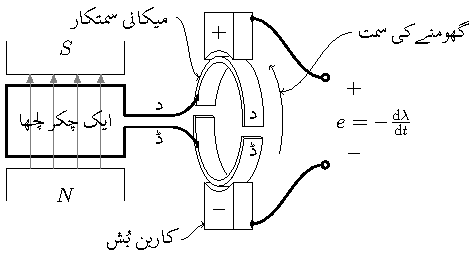
\includegraphics{figDCcommutatorA}
\caption{میکانی سمت کار۔}
\label{شکل_یکسمتی_میکانی_سمتکار}
\end{figure}

دکھائے گئے لمحہ پر لچھے میں پیدا برقی دباؤ \عددیء{e} کی وجہ سے لچھے کا برقی سرا د مثبت اور اس کا برقی سرا ڈ منفی ہے۔یوں سمت کار کا حصہ د مثبت اور اس کا حصہ ڈ منفی ہے جس سے کاربن کے \عددیء{+} نشان والا بُش مثبت اور \عددیء{-} نشان والا بُش منفی ہے۔
\begin{figure}
\centering
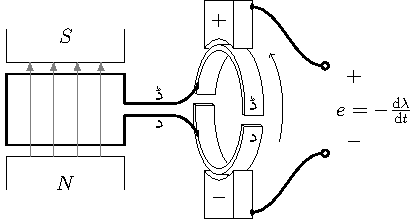
\includegraphics{figDCcommutatorB}
\caption{آدھے چکر کے بعد بھی \عددیء{+} بُش مثبت ہی ہے۔}
\label{شکل_یکسمتی_میکانی_سمتکار_آدھے_چکر_بعد}
\end{figure}
آدھے چکر بعد خلاء میں لچھے کی د اور ڈ اطراف آپس میں جگہیں تبدیل کر لیں گی۔یہ شکل \حوالہ{شکل_یکسمتی_میکانی_سمتکار_آدھے_چکر_بعد}  میں دکھایا گیا ہے۔لچھے کے د اور ڈ اطراف اب بھی سمت کار کے د اور ڈ حصوں کے ساتھ جُڑے ہیں۔ اس لمحہ پر لچھے پر برقی دباؤ اُلٹ ہو گی اور اب اس کا د طرف منفی اور ڈ طرف مثبت ہو گا جیسے شکل میں دکھایا گیا ہے۔یہاں سمت کار کی کارکردگی سامنے آتی ہے اور ہم دیکھتے ہیں کہ کاربن کا \عددیء{+}  نشان والا بُش اب بھی مثبت اور \عددیء{-} نشان والا بُش اب بھی منفی ہے۔ یوں جنریٹر کے بیرونی برقی سروں پر اب بھی برقی دباؤ پہلے کی سمت میں ہی ہے۔سمت کاری کے دانتوں کے مابین برقی دباؤ ہوتا ہے لہٰذا ان کو غیر موصل شہ کی مدد ایک دونوں سے اور دھرے سے دور رکھا جاتا ہے۔

گھومتے وقت ایک ایسا لمحہ آتا ہے جب سمت کار کے دونوں دانت کاربن کے دونوں بُشوں کے ساتھ جُڑے ہوتے ہیں یعنی اس لمحہ کاربن کے بُش لچھے کو کسرِ دور کرتے ہیں۔ کاربن کے بُش محیط پر اس طرح رکھے جاتے ہیں کہ جس لمحہ لچھے میں برقی دباؤ مثبت سے منفی یا منفی سے مثبت ہونے لگے اسی لمحہ کاربن کے بُش لچھے کو کسرِ دور کرے۔چونکہ اس لمحہ لچھے کے پیدا کردہ برقی دباؤ صفر ہوتی ہے لہٰذا اسے کسرِ دور کرنے سے کوئی نقصان نہیں ہوتا۔اس طرح حاصل برقی دباؤ شکل \حوالہ{شکل_یکسمتی_دو_دندوں_کا_سمتکار}  میں دکھایا گیا ہے۔
\begin{figure}
\centering
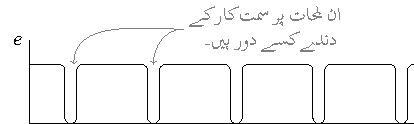
\includegraphics{figDCcommutatorVoltage}
\caption{دو دندوں کے سمت کار سے حاصل یک سمتی برقی دباؤ۔}
\label{شکل_یکسمتی_دو_دندوں_کا_سمتکار}
\end{figure}


یہاں دو دندوں والا سمت کار اور دو مقناطیسی قطب کے درمیان گھومتا ایک ہی قوی لچھا دکھایا گیا ہے۔حقیقت میں جنریٹر کے بہت سارے قطب ہوں گے اور ہر ایک قطب کے لئے سمت کار کے کئی دندے ہوں گے۔مزید یہ کہ نہایت چھوٹی آلوں میں مقناطیسی میدان مقناطیس ہی فراہم کرتا ہے جبکہ بڑی آلوں میں مقناطیسی میدان ساکن میدانی لچھے فراہم کرتے ہیں۔ مشین کے دونوں قسم کے لچھے تقسیم شدہ ہوتے ہیں۔

اب ہم زیادہ دندوں کے ایک سمت کار کو دیکھتے ہیں۔

\جزوحصہ{میکانی سمت کار کی تفصیل}
پچھلے حصہ میں سمت کار کی بنیادی کارکردگی سمجھائی گئی۔ اس حصہ میں اس پر تفصیلاً غور کیا جائے گا۔یہاں شکل \حوالہ{شکل_یکسمتی_سمتکار_بش_کسر_دور_نہیں_کر_رہا}  سے رجوع کریں۔اس شکل میں اندر کی جانب دکھائے گئے سمت کار کے دندوں کو ہندسوں سے ظاہر کیا گیا ہے۔سمت کار کی اندر جانب کاربن بُش دکھائے گئے ہیں جبکہ  بیرونِ جنریٹر برقی رو کو ظاہر کرتی ہے۔شگافوں کو بھی ہندسوں سے ظاہر کیا گیا ہے۔اس جنریٹر کے دو قطب ہیں جبکہ اس میں کُل آٹھ شگاف ہیں۔اس طرح اگر ایک شگاف ایک قطب کے سامنے ہو تو تین شگاف چھوڑ کر موجود شگاف دوسرے قطب کے سامنے ہو گا۔ہم کہتے ہیں کہ ایسے دو شگاف ایک قطب فاصلے پر ہیں مثلاً شگاف ایک اور پانچ ایک قطب کے فاصلے پر ہیں۔
\begin{figure}
\centering
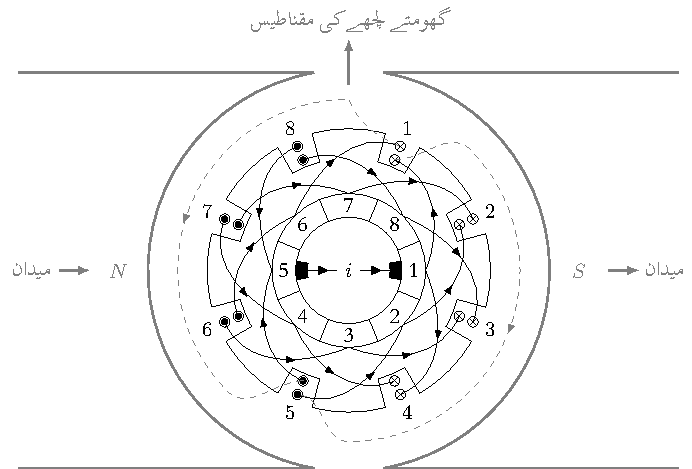
\includegraphics[scale=0.75]{figDCeightTeethCommutator}
\caption{کاربن بُش سمتکار کے دندوں کو کسرِ دور نہیں کر رہا۔}
\label{شکل_یکسمتی_سمتکار_بش_کسر_دور_نہیں_کر_رہا}
\end{figure}

شگافوں میں موجود لچھوں میں برقی رو کی سمتیں نقطہ اور صلیب سے ظاہر کئے گئے ہیں۔ نقطہ صفحہ سے عمودی طور پر باہر جانب کی سمت کو ظاہر کرتی ہے جبکہ صلیب کے نشان اس کی اُلٹ سمت کو ظاہر کرتی ہے۔یوں پہلی شگاف میں برقی رو کی سمت عمودی طور پر صفحہ کی اندر جانب کو ہے۔
\begin{figure}
\centering
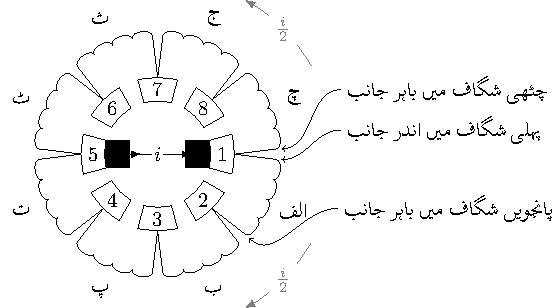
\includegraphics{figDCeightTeethCommutatorShowingCoilConnections}
\caption{سمت کار سے جڑے لچھے۔}
\label{شکل_یکسمتی_سمتکار_سے_جڑے_لچھے}
\end{figure}

ہر شگاف میں دو لچھے دکھائے گئے ہیں۔پہلی شگاف کی اندر جانب موجود لچھا، سمت کار کی پہلی دانت سے جُڑا ہے۔یہ جوڑ موٹی لکیر سے ظاہر کی گئی ہے۔شگاف کے نچلے سرے سے نکل کر یہ لچھا پانچ نمبر شگاف کے نچلے سرے میں باہر جانب کو داخل ہوتا ہے۔اس بات کو نقطہ دار لکیر سے دکھایا گیا ہے۔اسی طرح دو لچھے دوسرے اور چٹے شگافوں میں ہیں۔ان میں ایک لچھا دوسرے شگاف میں اندر کی جانب اور چٹے شگاف میں باہر کی جانب ہے جبکہ دوسرا لچھا دوسرے شگاف میں باہر کی جانب اور چٹے شگاف میں اندر کی جانب ہے۔ نقطہ دار لکیریں صرف پہلی اور پانچویں شگاف کے لئے دکھائے گئے ہیں۔آپ خود باقی شگافوں کے لئے انہیں بنا سکتے ہیں۔ہر لچھے کی ایک طرف شگاف میں اندر جانب  اور اس کی دوسری طرف ایک قطب دور موجود شگاف میں باہر جانب کو ہوتی ہے۔سمت کار کا یہی پہلا دانت چوتھے شگاف کی باہر جانب موجود لچھے سے بھی جُڑا ہے۔آپ یہاں رکھ کر شکل \حوالہ{شکل_یکسمتی_سمتکار_سے_جڑے_لچھے}  کی مدد سے مشین میں برقی رو کی سمتیں سمجھیں اور تسلی کر لیں کہ یہ درست دکھائے گئے ہیں۔اس شکل میں لچھوں کو الف، ب ، پ وغیرہ نام دیئے گئے ہیں جبکہ سمت کار کے دندوں کو ہندسوں سے ظاہر کیا گیا ہے۔کاربن کے بُش پہلے اور پانچویں دانت سے جڑے دکھائے گئے ہیں۔

اس شکل میں کاربن بُش سے برقی رو سمت کار کی پہلے دانت سے ہوتے ہوئے دو برابر مقداروں میں تقسیم ہو کر دو یکساں متوازی راستوں گزرے گی۔ایک راستہ سلسلہ وار جڑے الف، ب، پ اور ت لچھوں سے بنتا ہے جبکہ دوسرا راستہ سلسلہ وار جڑے ٹ، ث، ج اور چ لچھوں سے بنتا ہے۔یہ دو سلسلہ وار راستے آپس میں متوازی جڑے ہیں۔برقی رو کی سمت نقطہ دار چونچ والی لکیر سے ظاہر کی گئی ہے۔دو متوازی راستوں سے گزرتا برقی رو ایک مرتبہ دوبارہ مل کر ایک ہو جاتا ہے اور سمت کار کے پانچویں دانت سے جڑے کاربن بُش کے ذریعہ مشین سے باہر نکل جاتا ہے۔ آپ دیکھ سکتے ہیں کہ گھومتے حصے کی شگافوں میں موجود لچھوں میں برقی رو مقناطیسی دباؤ کو جنم دے گی جو ساکن مقناطیسی دباؤ کی عمودی سمت میں ہو گی جیسا شکل \حوالہ{شکل_یکسمتی_سمتکار_بش_کسر_دور_نہیں_کر_رہا}  میں دکھایا گیا ہے۔یہ دو مقناطیسی دباؤ دھرے پر گھڑی کی سمت میں قوت گردشہ پیدا کریں گے۔یوں اگر مشین موٹر کے طور پر استعمال کی جا رہی ہو تو یہ گھڑی کی سمت گھومے گی۔اس صورت میں کاربن بُش پر بیرونی یک سمتی برقی دباؤ اس سمت میں لاگو کی جائے گی کہ اس میں برقی رو دکھلائی گئی سمت میں ہو۔
\begin{figure}
\centering
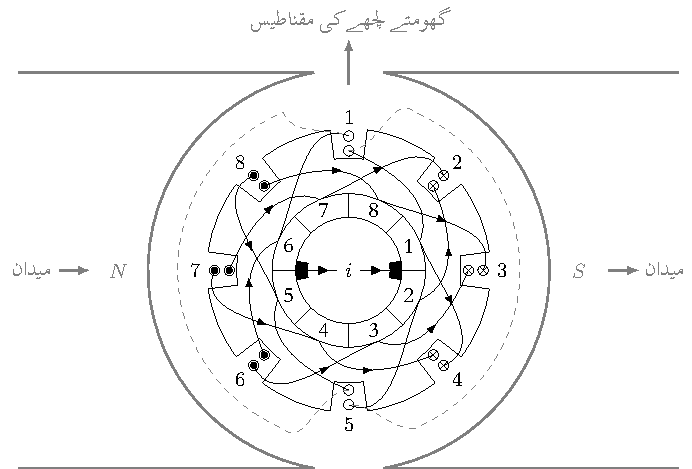
\includegraphics[scale=0.75]{figDCeightTeethCommutatorShortingAcoil}
\caption{کاربن بُش سمت کار کے دندوں کو کسرِ دور کر رہا ہے۔}
\label{شکل_یکسمتی_سمتکار_کے_دندے_کسرے_دور}
\end{figure}

اب یہ تصور کریں کہ مشین ایک جنریٹر کے طور پر استعمال کی جا رہی ہو اور اسے گھڑی کی اُلٹی سمت بیرونی میکانی طاقت سے گھمایا جا رہا ہو۔یوں سمت کار کے آدھے دانت برابر حرکت کرنے کے بعد یہ شکل \حوالہ{شکل_یکسمتی_سمتکار_کے_دندے_کسرے_دور} میں دکھلائے حالت اختیار کر لے گی۔اس شکل میں دائیاں کاربن بُش سمت کار کے پہلے اور دوسرے دانت کے ساتھ جبکہ بائیاں کاربن بُش اس کے پانچویں اور چھٹے دانت کے ساتھ جُڑ گئے ہیں۔یوں پہلے اور پانچویں شگافوں میں موجود لچھے کسرِ دور ہو گئے ہیں جبکہ بقایا شگافوں میں موجود لچھوں میں حسبِ معمول برقی رو ہو گا جن سے مقناطیسی دباؤ اب بھی پہلے کی طرح ساکن مقناطیسی کی دباؤ کی عمودی سمت میں ہو گا۔اس لمحہ کی صورت شکل \حوالہ{شکل_یکسمتی_دندے_کسرے_دور}  میں زیادہ واضح ہے۔
\begin{figure}
\centering
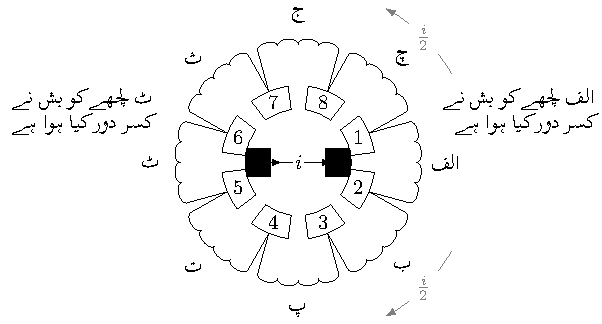
\includegraphics{figDCeightTeethCommutatorShowingCoilConnectionsShortedCoil}
\caption{کاربن بش دو دندوں کو کسر دور کر رہے ہیں۔}
\label{شکل_یکسمتی_دندے_کسرے_دور}
\end{figure}

مشین جب سمت کار کے ایک دانت برابر حرکت کر لے تو کاربن کے بُش دوسرے اور چھٹے دانت سے جُڑ جائیں گے۔پہلے اور پانچویں شگافوں میں برقی رو کی سمت پہلی سے اُلٹ ہو جائے گی جبکہ باقی شگافوں میں برقی رو کی سمتیں برقرار رہیں گی۔گھومتے لچھوں کا برقی دباؤ اب بھی اُسی سمت میں ہو گا۔

جتنے لمحے کے لئے  کاربن کے بُش دو لچھوں کو کسرِ دور کرتے ہیں اتنے وقت میں ان لچھوں میں برقی رو کی سمت اُلٹ ہو جاتی ہے۔کوشش کی جاتی ہے کہ  اس دوران برقی رو وقت کے ساتھ بتدریج تبدیل ہو۔ایسا نہ ہونے سے کاربن کے بُش سے چنگاریاں نکلتی ہیں جن سے یہ بُش جلد ناکارہ ہو جاتے ہیں۔جنریٹر کے کسر دور لچھوں میں پیدا برقی دباؤ انہیں لچھوں میں گھومتی برقی رو پیدا کرتی ہے جو ہمارے کسی کام کی نہیں۔لچھے اور کاربن بش کے برقی مزاحمت اس برقی رو کی قیمت کا تعین کرتے ہیں۔ 

حقیقت میں یک سمتی جنریٹر میں درجن دانت فی قطب والا سمت کار استعمال ہو گا اور اگر مشین نہایت چھوٹی نہ ہو تو اس میں دو سے زیادہ قطب ہوں گے۔


%======================
\حصہ{یک سمتی جنریٹر کی برقی دباؤ}
گزشتہ حصہ میں شکل \حوالہ{شکل_یکسمتی_سمتکار_سے_جڑے_لچھے} کے الف، ب، پ اور ت لچھے سلسلہ وار جڑے ہیں۔ اسی طرح ٹ، ث، ج اور چ لچھے سلسلہ وار جڑے ہیں۔حصہ \حوالہ{حصہ_گھومتے_مشین_محرک_برقی_دباؤ}  میں مساوات \حوالہ{مساوات_گھومتے_مشین_پیدا_دباؤ}  ایک لچھے کی یک سمتی جنریٹر کی محرک برقی دباؤ \عددیء{e_1} دیتی ہے۔ اسے یہاں یاد دھیانی کی خاطر دوبارہ دیا جاتا ہے۔
\begin{align}\label{مساوات_یکسمتی_پیدا_دباؤ_دوبارہ}
e_1=\omega N \phi_m=\omega N A B_m
\end{align}
اگر خلائی درز میں \عددیء{B_m} کی مقدار ہر جگہ یکساں ہو تو سب لچھوں میں برابر محرک برقی دباؤ پیدا ہو گا۔یوں شکل \حوالہ{شکل_یکسمتی_سمتکار_بش_کسر_دور_نہیں_کر_رہا}  میں دکھائے لمحہ پر جنریٹر کی کُل محرک برقی دباؤ \عددیء{e} ایک لچھے کی محرک برقی دباؤ کی چار گنا ہو گی یعنی
\begin{gather}
\begin{aligned}
e&=e_{\textup{الف}}+e_{\textup{ب}}+e_{\textup{پ}}+e_{\textup{ت}}  \\
&=e_{\textup{ٹ}}+e_{\textup{ث}}+e_{\textup{ج}}+e_{\textup{چ}}  \\
&=4 \omega N A B_m
\end{aligned}
\end{gather}
جبکہ شکل \حوالہ{شکل_یکسمتی_سمتکار_کے_دندے_کسرے_دور}  میں دکھائے لمحہ پر صرف تین لچھوں کی محرکی برقی دباؤ زیرِ استعمال آتی ہے یعنی
\begin{gather}
\begin{aligned}
e&=e_{\textup{ب}}+e_{\textup{پ}}+e_{\textup{ت}}  \\
&=e_{\textup{ث}}+e_{\textup{ج}}+e_{\textup{چ}}  \\
&=3 \omega N A B_m
\end{aligned}
\end{gather}
%

\begin{figure}
\centering
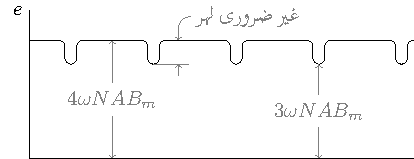
\includegraphics{figDCrippleInVoltage}
\caption{آٹھ دندوں کی میکانی سمت کار سے حاصل برقی دباؤ۔}
\label{شکل_یکسمتی-آٹھ_دندوں_سمتکار_کی_لہر}
\end{figure}

شکل \حوالہ{شکل_یکسمتی-آٹھ_دندوں_سمتکار_کی_لہر}  میں اس آٹھ دندوں والے میکانی سمت کار سے حاصل برقی دباؤ دکھائی گئی ہے۔اس شکل میں یک سمتی برقی دباؤ پر سوار غیر ضروری لہریں نظر آ رہی ہیں۔اگر جنریٹر میں ایک جوڑی قطب پر کُل \عددیء{n} لچھے ہوں تو شکل \حوالہ{شکل_یکسمتی_سمتکار_سے_جڑے_لچھے}  کی طرح یہ دو \عددیء{\tfrac{n}{2}}  سلسلہ وار لچھوں جتنی محرکی برقی دباؤ پیدا کرے گی۔
\begin{align}\label{مساوات_یکسمتی_پیدا_دباؤ_الف}
e=\frac{n}{2} \omega N \phi_m=\frac{n}{2} \omega N A B_m
\end{align}
اس صورت میں یہ غیر ضروری لہریں کُل یک سمتی برقی دباؤ کی تقریباً
\begin{align}\label{مساوات_یکسمتی_فی_صد_لہر}
\frac{\omega N \phi_m}{\frac{n}{2} \omega N \phi_m} \times 100=\frac{2}{n} \times 100
\end{align}
فی صد ہو گی۔آپ دیکھ سکتے ہیں کہ اگر فی قطب دندوں کی تعداد بڑھائی جائے تو حاصل برقی دباؤ زیادہ ہموار ہو گی اور یہ غیر ضروری لہریں قابلِ نظر انداز ہوں گے۔

اب تصور کریں کہ شکل \حوالہ{شکل_یکسمتی_سمتکار_بش_کسر_دور_نہیں_کر_رہا}  میں دیئے مشین کی خلائی درز میں \عددیء{B_m} کی مقدار ہر جگہ یکساں نہیں ہے۔اس صورت میں لچھوں میں محرک برقی دباؤ مساوات \حوالہ{مساوات_یکسمتی_پیدا_دباؤ_دوبارہ}  کے تحت مختلف زاویوں پر مختلف ہو گی۔اس طرح مشین سے حاصل کُل برقی دباؤ چار سلسلہ وار لچھوں کی مختلف محرک برقی دباؤ کے مجموعہ کے برابر ہو گی یعنی
\begin{align} \label{مساوات_یکسمتی_کل_دباؤ_مجموعہ}
e=e_1+e_2+e_3+e_4
\end{align}
جہاں  \عددیء{e_1,e_2,\cdots} مختلف لچھوں کی محرک برقی دباؤ کو ظاہر کرتے ہیں۔

اب شکل  \حوالہ{شکل_یکسمتی_سمتکار_بش_کسر_دور_نہیں_کر_رہا} پر غور کریں۔اگر گھومتا حصہ صرف ایک دندے برابر حرکت کرے تو اس شکل کی حالت  دوبارہ حاصل ہوتی ہے اور اس سے حاصل برقی دباؤ بھی دوبارہ وہی ملتی ہے۔اگر میکانی سمت کار کی فی قطب دندوں کی تعداد زیادہ کر دی جائے تو یہ حرکت قابلِ نظر انداز ہو جاتی ہے۔ اب اگر خلائی درز میں کثافتِ مقناطیسی بہاو ہمواری کے ساتھ تبدیل ہو تو اتنی کم حرکت کے احاطے میں \عددیء{B_m} کی مقدار میں کوئی خاص تبدیلی نہیں آئے گی اور اس احاطے میں اسے یکساں تصور کیا جا سکتا ہے۔یوں اگر لچھا اس احاطے میں حرکت کرے تو اس میں محرک برقی دباؤ تبدیل نہیں ہو گی۔یعنی جس لچھے کی محرکی برقی دباؤ \عددیء{e_1} ہے اُس کی اس احاطے میں محرکی برقی دباؤ یہی رہے گی۔یوں اگرچہ \عددیء{e_1,e_2,\cdots} آپس میں مختلف ہو سکتے ہیں مگر ان کی مقدار قطعی ہے، لہٰذا اس صورت میں مساوات \حوالہ{مساوات_یکسمتی_کل_دباؤ_مجموعہ}  میں دی گئی محرکی برقی دباؤ کی مقدار بھی قطعی ہو گی۔ 

ہم نے دیکھا کہ اگر خلائی درز میں \عددیء{B_m} ہمواری کے ساتھ تبدیل ہو تو جنریٹر سے معیاری یک سمتی محرک برقی دباؤ حاصل ہوتی ہے۔بدلتی رو جنریٹروں میں \عددیء{B_m} سائن نما رکھنی ضروری ہوتی ہے۔نہایت چھوٹی یک سمتی آلوں میں خلائی درز میں \عددیء{B_m}  یکساں رکھا جاتا ہے جبکہ بڑی آلوں میں اسے ہمواری کے ساتھ تبدیل کیا جاتا ہے۔جیسا اوپر ذکر ہوا عملاً میکانی سمت کار کے دندوں تک لچھوں کے سروں کی رسائی ممکن تب ہوتی ہے جب ہر شگاف میں دو لچھے رکھے جائیں۔ اس طرح رکھے لچھوں کی خلائی درز میں مقناطیسی دباؤ آری کے دندوں کی مانند ہوتا ہے۔یہ شکل \حوالہ{شکل_یکسمتی_آری_دندوں_نما_دباؤ}  میں دکھایا گیا ہے۔
\begin{figure}
\centering
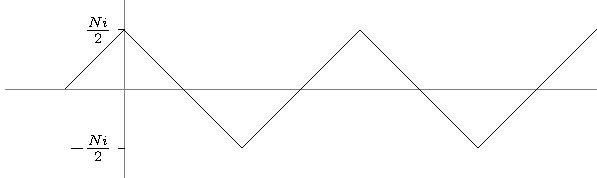
\includegraphics{figDCsawtoothMMF}
\caption{آری دندوں نما کثافتِ مقناطیسی دباؤ۔}
\label{شکل_یکسمتی_آری_دندوں_نما_دباؤ}
\end{figure}

زیادہ قطب کے مشین میں شمالی اور جنوبی قطب کے ایک جوڑے کی پیدا یک سمتی برقی دباؤ مساوات \حوالہ{مساوات_یکسمتی_پیدا_دباؤ_الف}  سے حاصل ہو گی جہاں \عددیء{n} ایک قطبین کے جوڑے پر میکانی سمت کار کے دندوں کی تعداد ہو گی۔یوں زیادہ قطبین کے جوڑیوں سے حاصل یک سمتی برقی دباؤ کو سلسلہ وار یا متوازی جوڑا جا سکتا ہے۔

\حصہ{قوت گردشہ}
یک سمتی آلوں کی امالی برقی دباؤ اور قوت گردشہ خلائی درز میں مقناطیسی دباؤ کی شکل پر منحصر نہیں۔اپنی سہولت کے لئے ہم ان کی خلائی درز میں مقناطیسی دباؤ سائن نما تصور کرتے ہیں۔شکل \حوالہ{شکل_یکسمتی_آری_دندوں_نما_دباؤ}  میں دکھائے گئے قوی لچھے کی مقناطیسی دباؤ کی بنیادی فوریئر جزو\فرہنگ{فورئیر}\حاشیہب{fundamental Fourier component}
\begin{align}
\tau_q=\frac{8}{\pi^2} \frac{N I}{2}
\end{align}
ہے۔یوں چونکہ یک سمتی مشین میں ساکن اور گھومتے لچھوں کی مقناطیسی دباؤ عمودی ہیں لہٰذا ان میں قوت گردشہ مساوات \حوالہ{مساوات_گھومتے_مشین_مروڑ_اور_بہاو}  کی طرح
\begin{align}\label{مساوات_یکسمتی_مروڑ}
T=-\frac{\pi}{2}\left( \frac{P}{2}\right)^2 \phi_m \tau_q 
\end{align} 
ہو گی۔
%
\ابتدا{مثال}
دو قطب بارہ دندوں کے میکانی سمت کار کے یک سمتی جنریٹر میں ہر قوی لچھا بیس چکر کا ہے۔ایک لچھے سے گزرتی مقناطیسی بہاو  \عددیء{0.0442} ویبر ہے۔جنریٹر \عددیء{3600} چکر فی منٹ کی رفتار سے گھوم رہا ہے۔
\begin{itemize}
\item
اس کی پیدا یک سمتی برقی دباؤ میں غیر ضروری لہریں کُل برقی دباؤ کے کتنے فی صد ہیں۔
\item
یک سمتی برقی دباؤ حاصل کریں۔
\end{itemize}

حل:
\begin{itemize}
\item
مساوات \حوالہ{مساوات_یکسمتی_فی_صد_لہر}  سے غیر ضروری لہریں \عددیء{\tfrac{2}{n} \times 100=\tfrac{2}{12}\times 100=16.66} فی صد ہیں۔
\item
جنریٹر کی رفتار \عددیء{\tfrac{3600}{60}=60} ہرٹز ہے یوں مساوات \حوالہ{مساوات_یکسمتی_پیدا_دباؤ_الف}  کی مدد سے حاصل یک سمتی برقی دباؤ
\begin{align*}
e=\frac{12}{2} \times 2 \times \pi \times 60 \times 20 \times 0.0442=\SI{1999.82}{\volt}
\end{align*}
ہے۔
\end{itemize}
\انتہا{مثال}
%
\حصہ{بیرونی ہیجان  اور خود ہیجان یک سمتی جنریٹر}
\اصطلاح{بیرونی ہیجان}\فرہنگ{ہیجان!بیرونی}\حاشیہب{separately excited}\فرہنگ{separately excited} یک سمتی جنریٹر کے میدانی لچھے کو بیرونی یک سمتی برقی دباؤ مہیا کی جاتی ہے جبکہ \اصطلاح{خود ہیجان}\فرہنگ{ہیجان!خود}\حاشیہب{self excited}\فرہنگ{self excited} یک سمتی جنریٹر کے میدانی لچھے کو اس جنریٹر کی اپنی پیدا کردہ محرک برقی دباؤ ہی مہیا کی جاتی ہے۔یک سمتی جنریٹر کی کارکردگی اس کو ہیجان کرنے کے طریقے پر منحصر ہے۔
\begin{figure}
\centering
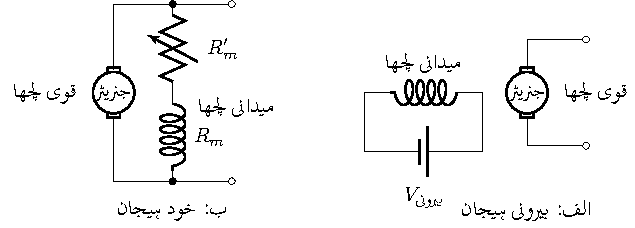
\includegraphics{figDCselfExcitedAndSeparatelyExcited}
\caption{بیرونی ہیجان اور خود ہیجان یک سمتی جنریٹر۔}
\label{شکل_یکسمتی_خود_ہیجان_بیرونی_ہیجان}
\end{figure}

شکل \حوالہ{شکل_یکسمتی_خود_ہیجان_بیرونی_ہیجان}-الف میں قوی لچھے\فرہنگ{قوی لچھے}\حاشیہب{armature coil}\فرہنگ{armature coil} اور میدانی لچھے\فرہنگ{میدانی لچھے}\حاشیہب{filed coil}\فرہنگ{field coil} کو آپس میں عمودی بنایا گیا ہے۔ یہ ایک سادہ طریقہ ہے جس سے یہ یاد رہتا ہے کہ ان لچھوں کی پیدا کردہ مقناطیسی دباؤ عمودی ہیں۔یہاں قوی لچھے کی شکل میکانی سمت کار کی طرح بنائی گئی ہے۔

چونکہ میدانی اور قوی لچھوں کی مقناطیسی دباؤ عمودی ہیں ہم اس سے یہ اخذ کرتے ہیں کہ ایک لچھے کی برقی دباؤ دوسرے لچھے کی برقی دباؤ پر اثر انداز نہیں ہوتی۔اس کا مطلب ہے کہ مقناطیسی مرکز کی کسی ایک سمت میں  سیرابیت اس سمت کی عمودی سمت میں سیرابیت پر اثر انداز نہیں ہوتی۔

\begin{figure}
\centering
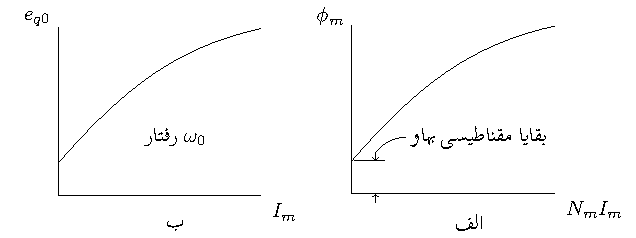
\includegraphics[width=\linewidth]{figDCBrillouinFunctionGeneratedVoltageVersusFieldCurrent}
\caption{میدانی برقی رو سے محرکی برقی دباؤ قابو کی جاتی ہے۔}
\label{شکل_یکسمتی_پیدا_برقی_دباؤ_بالمقابل_میدانی_رو}
\end{figure}
شکل \حوالہ{شکل_یکسمتی_خود_ہیجان_بیرونی_ہیجان}-الف میں بیرونی ہیجان مشین کی میدانی لچھے کو بیرونی یک سمتی برقی طاقت مہیا کی گئی ہے۔یوں میدانی لچھے کی برقی رو تبدیل کر کے اس کی میدانی مقناطیسی دباؤ  \عددیء{\tau_m}، میدانی مقناطیسی بہاو \عددیء{\phi_m}  اور کثافتِ مقناطیسی بہاو \عددیء{B_m}  تبدیل کی جا سکتی ہے۔یوں جنریٹر کی محرک برقی دباؤ مساوات \حوالہ{مساوات_یکسمتی_پیدا_دباؤ_دوبارہ}  کے تحت تبدیل کی جا سکتی ہے یا پھر موٹر کی قوت گردشہ مساوات \حوالہ{مساوات_یکسمتی_مروڑ}  کے تحت تبدیل کی جا سکتی ہے۔

برقی رو بڑھانے سے مرکز کا سیراب ہونا شکل \حوالہ{شکل_یکسمتی_پیدا_برقی_دباؤ_بالمقابل_میدانی_رو}  میں واضح ہے۔یوں برقی رو بڑھاتے ہوئے شروع میں محرک برقی دباؤ اور میدانی لچھے کی برقی رو براہِ راست متناسب ہو گی جبکہ زیادہ برقی رو پر ایسا نہیں۔شکل میں خط ب مشین کے کُھلے سرے معائنہ سے حاصل کی جا سکتی ہے۔اس شکل میں محرکی برقی دباؤ کو \عددیء{e} کی بجائے  \عددیء{e_{q0}} لکھ کر اس بات کی یاد دھیانی کرائی گئی ہے کہ یہ محرکی دباؤ  قوی لچھے سے حاصل کی گئی ہے اور یہ ایک معین رفتار \عددیء{\omega_0} پر حاصل کی گئی ہے۔اگر کسی اور رفتار \عددیء{\omega} پر اس خط سے محرکی برقی دباؤ \عددیء{e_q} حاصل کرنی ہو تو مساوات \حوالہ{مساوات_یکسمتی_پیدا_دباؤ_الف}  کی مدد سے
\begin{align}
\frac{e_q}{e_{q0}}=\frac{\frac{n}{2} \omega N A B_m}{\frac{n}{2} \omega_0 N A B_m}=\frac{\omega}{\omega_0}
\end{align}
یعنی
\begin{align}\label{مساوات_یکسمتی_چکر_بالمقابل_رفتار}
e_q=\frac{rpm}{rpm_0} e_{q0}
\end{align}
جہاں رفتار کو چکر فی منٹ\حاشیہب{rpm, rounds per minute} میں بھی لیا گیا ہے۔یاد رہے کہ یہ مساوات صرف اُس صورت میں درست ہے جب مقناطیسی میدان تبدیل نہ ہو۔

مقناطیسی مرکز اگر مقناطیس بنائی جائے تو اس میں بقایا مقناطیسی بہاو رہتی ہے۔یہ شکل کے حصہ الف میں دکھائی گئی ہے۔یوں اگر میدانی لچھے کو ہیجان نہ بھی کیا جائے تو جنریٹر کچھ محرکی برقی دباؤ پیدا کرے گی\حاشیہد{آپ ٹھیک سوچ رہے ہیں۔جنریٹر بنانے والے کارخانے میں مرکز کو پہلی مرتبہ مقناطیس بنانا پڑتا ہے}۔ یہ بقایا  محرکی برقی دباؤ شکل ب میں صفر میدانی برقی رو پر دکھائی گئی ہے۔

 اگر خود ہیجان جنریٹر کو ساکن حال سے چالو کیا جائے تو بقایا محرکی برقی دباؤ پیدا ہو گی۔اس محرک برقی دباؤ سے میدانی لچھے میں برقی رو رواں ہو گا اور یوں مقناطیسی میدان پیدا ہو گا جس سے مشین ذرا زیادہ ہیجان ہو جائے گا اور یوں اس کی محرکی برقی دباؤ بھی کچھ بڑھ جائے گی۔اس طرح کرتے کرتے مشین جلد پوری محرک برقی دباؤ پیدا کرنے شروع ہوتا ہے۔یہ سب اسی اثنا میں ہوتا ہے جب مشین کی رفتار بڑھ رہی ہوتی ہے۔

شکل \حوالہ{شکل_یکسمتی_خود_ہیجان_بیرونی_ہیجان}-ب میں خود ہیجان مشین دکھائی گئی ہے جس کے میدانی اور قوی لچھے متوازی جُڑے ہیں۔ اس طرح جڑی جنریٹر کو \اصطلاح{خود ہیجان  متوازی جڑی}\فرہنگ{داخلی ہیجان!متوازی}\حاشیہب{parallel connected}\فرہنگ{parallel connected} جنریٹر کہتے ہیں۔اس شکل میں میدانی لچھے کے ساتھ ایک مزاحمت سلسلہ وار جڑی ہے۔اس مزاحمت کو تبدیل کر کے میدانی برقی رو تبدیل کی جاتی ہے جس سے بالکل بیرونی ہیجان مشین کی طرح جنریٹر کی محرکی برقی دباؤ یا موٹر کی قوت گردشہ تبدیل کی جاتی ہے۔
\begin{figure}
\centering
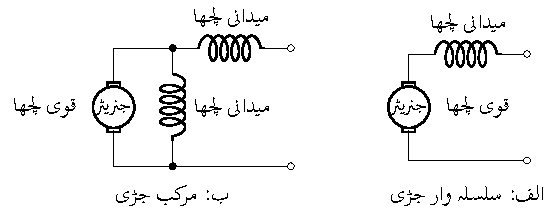
\includegraphics{figDCseriesAndCompound}
\caption{سلسلہ وار اور مرکب جڑی خود ہیجان جنریٹر۔}
\label{شکل_یکسمتی_سلسلہ_وار_اور_مرکب}
\end{figure}

شکل \حوالہ{شکل_یکسمتی_سلسلہ_وار_اور_مرکب}  میں خود ہیجان جنریٹر کی دو اور قسمیں دکھائی گئی ہیں۔ ایک \اصطلاح{خود ہیجان  سلسلہ وار جڑی} جنریٹر\فرہنگ{داخلی ہیجان!سلسلہ وار}  اور \اصطلاح{دوسری خود ہیجان  مرکب} جنریٹر\فرہنگ{داخلی ہیجان!مرکب}  ہے۔سلسلہ وار جڑی جنریٹر میں میدانی اور قوی لچھے سلسلہ وار جُڑے ہوتے ہیں۔\اصطلاح{مرکب جنریٹر}\فرہنگ{مرکب جنریٹر} میں میدانی لچھے کے دو حصے ہوتے ہیں جن میں ایک قوی لچھے کے متوازی اور دوسرا اس کے سلسلہ وار جُڑے ہوتے ہیں۔مزید یہ کہ متوازی جُڑا حصہ قوی لچھے کے قریب ہو سکتا ہے یا پھر یہ سلسلہ وار لچھے کے دوسری جانب یعنی دور جُڑا ہو سکتا ہے۔پہلی صورت میں اسے \اصطلاح{قریب جڑی مرکب} جنریٹر\فرہنگ{قریب جڑی مرکب} اور دوسری صورت میں \اصطلاح{دور جڑی مرکب} جنریٹر\فرہنگ{دور جڑی مرکب} کہیں گے۔شکل \حوالہ{شکل_یکسمتی_قریب_دور_جڑی_جنریٹر}  میں مرکب جنریٹر کے دونوں اشکال دکھائے گئے ہیں۔ 
\begin{figure}
\centering
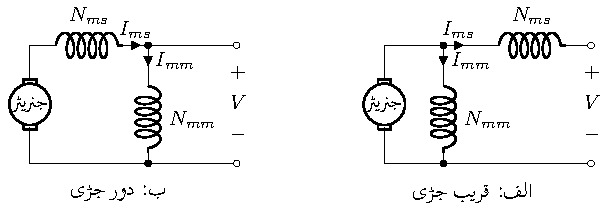
\includegraphics{figDCnearAndFarConnected}
\caption{مرکب قریب جڑی اور مرکب دور جڑی خود ہیجان جنریٹر}
\label{شکل_یکسمتی_قریب_دور_جڑی_جنریٹر}
\end{figure}

یک سمتی موٹر بھی اسی طرح پکارے جاتے ہیں۔یعنی شکل \حوالہ{شکل_یکسمتی_خود_ہیجان_بیرونی_ہیجان}  کی طرح جڑی دو موٹروں کو بیرونی ہیجان موٹر اور خود ہیجان متوازی جڑی موٹر کہیں گے۔موٹر میں قوی لچھے کی برقی رو کی سمت جنریٹر کے برقی رو کی سمت کے اُلٹ ہوتی ہے۔

ہر طرح جڑی یک سمتی جنریٹر کی میدانی مقناطیسی دباؤ اس کے میدانی لچھے کے چکر ضرب برقی رو کے برابر ہوتی ہے یعنی
\begin{align}
\tau=N_m I_m
\end{align}
شکل  \حوالہ{شکل_یکسمتی_خود_ہیجان_بیرونی_ہیجان} میں خود ہیجان متوازی جڑی جنریٹر کی میدانی لچھے میں برقی رو اس لچھے اور اس کے ساتھ جڑی مزاحمت کے مجموعہ  مزاحمت \عددیء{R=R_m+R_m'} پر منحصر ہو گی یعنی \عددیء{I_m=\tfrac{V}{R}} یوں خود ہیجان متوازی جڑی جنریٹر کے لئے اس مساوات کو یوں لکھا جائے گا۔
\begin{align}
\tau_{m,m}=\frac{I_m V}{R_m+R_m'}
\end{align}
سلسلہ وار جڑی جنریٹر میں میدانی برقی رو جنریٹر کے قوی لچھے کی برقی رو کے برابر ہوتی ہے لہٰذا اس صورت میں اس مساوات کو یوں لکھا جا سکتا ہے۔
\begin{align}
\tau_{m,s}=N_m I_q
\end{align}
شکل \حوالہ{شکل_یکسمتی_قریب_دور_جڑی_جنریٹر}  میں مرکب جنریٹر میں میدانی مقناطیسی دباؤ کے دو حصے ہیں۔اس میں \عددیء{N_{mm}} چکر کے متوازی جڑے میدانی لچھے میں برقی رو \عددیء{I_{mm}}  اور  \عددیء{N_{ms}} چکر کے سلسلہ وار جڑے میدانی لچھے میں  برقی رو \عددیء{I_{ms}} ہے لہٰذا
\begin{align}
\tau_{m,mk}=N_{ms} I_{ms}+N_{mm} I_{mm}
\end{align}

\حصہ{یک سمتی مشین کی کارکردگی کے خط}
\جزوحصہ{حاصل برقی دباؤ بالمقابل برقی بوجھ}
مختلف طریقوں سے جُڑے یک سمتی جنریٹروں سے حاصل برقی دباؤ بمقابلہ ان پر لدے برقی بوجھ کے خط شکل \حوالہ{شکل_یکسمتی_محرک_دباؤ_بالمقابل_بار}  میں دکھائے گئے۔گھومتی رفتار معین تصور کی گئی ہے۔دھرے پر لاگو بیرونی میکانی طاقت جنریٹر کی قوت گردشہ کے خلاف اسے گھمائے گی۔
\begin{figure}
\centering
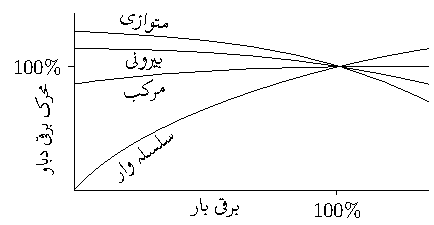
\includegraphics{figDCgeneratedVoltageVersusLoad}
\caption{یک سمتی جنریٹر کی محرک برقی دباؤ بمقابلہ برقی بوجھ کے خط۔}
\label{شکل_یکسمتی_محرک_دباؤ_بالمقابل_بار}
\end{figure}

ان خط کو سمجھنے کی خاطر پہلے بیرونی ہیجان جنریٹر پر غور کرتے ہیں جس کی مساوی برقی دور شکل \حوالہ{شکل_یکسمتی_خارجی_ہیجان_کا_مساوی}-الف میں دی گئی ہے۔بیرونی ہیجان جنریٹر پر برقی بوجھ لادنے سے اس کے قوی لچھے کی مزاحمت\حاشیہد{علامت Rq  کے زیر نوشت میں q لفظ قوی کے پہلی حرف ق کو ظاہر کرتی ہے ۔} \عددیء{R_q} میں برقی رو  \عددیء{I_q} گزرنے سے اس میں برقی دباؤ گھٹتی ہے۔لہٰذا جنریٹر سے حاصل برقی دباؤ \عددیء{V}، جنریٹر کی اندرونی محرک برقی دباؤ \عددیء{E_q}  سے قدرِ کم ہوتی ہے یعنی
\begin{align}
V=E_q-I_q R_q
\end{align}
برقی بوجھ \عددیء{I_q} بڑھانے سے جنریٹر سے حاصل برقی دباؤ کم ہو گی۔شکل میں بیرونی ہیجان جنریٹر کی خط ایسا ہی رجحان ظاہر کرتی ہے۔حقیقت میں کچھ اور وجوہات بھی کار آمد ہوتے ہیں جن سے یہ خط سیدھی نہیں بلکہ جھکی ہوتی ہے۔ 
\begin{figure}
\centering
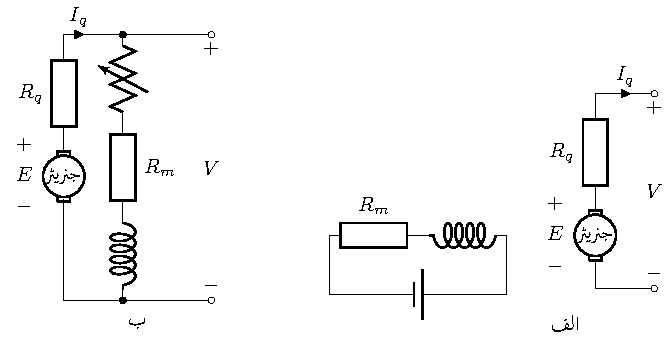
\includegraphics{figDCseparateExcitedEquivalentCircuit}
\caption{بیرونی ہیجان اور متوازی جڑی جنریٹر کی مساوی برقی دور۔}
\label{شکل_یکسمتی_خارجی_ہیجان_کا_مساوی}
\end{figure}

متوازی جڑی جنریٹر کے خط کا یہی رجحان ہے۔ متوازی جڑی جنریٹر پر بھی برقی بوجھ لادنے سے قوی لچھے کی مزاحمت میں برقی دباؤ گھٹتی ہے ۔یوں اس کے میدانی لچھے پر لاگو برقی دباؤ کم ہو جاتی ہے جس سے میدانی لچھے میں برقی رو بھی گھٹتی ہے۔ اس سے محرک برقی دباؤ مزید کم ہوتی ہے۔اس طرح ان جنریٹر سے حاصل برقی دباؤ بمقابلہ برقی بوجھ کے خط کی ڈھلان بیرونی ہیجان جنریٹر کی خط سے زیادہ ہوتی ہے۔
\begin{figure}
\centering
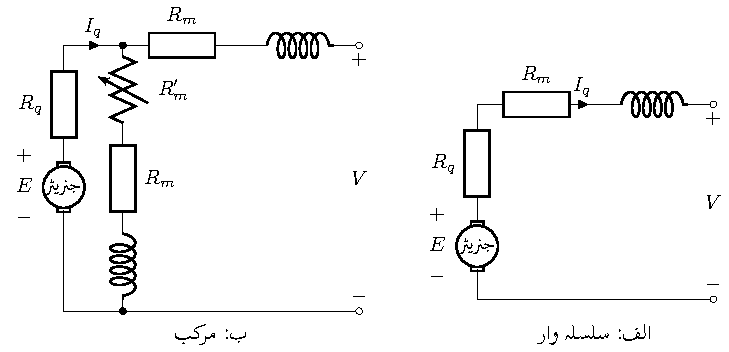
\includegraphics{figDCseriesAndCompoundEquivalentCircuit}
\caption{سلسلہ وار اور مرکب جنریٹر کے مساوی برقی دور۔}
\label{شکل_یکسمتی_سلسلہ_وار_اور_مرکب_مساوی}
\end{figure}

شکل \حوالہ{شکل_یکسمتی_سلسلہ_وار_اور_مرکب_مساوی}  میں سلسلہ وار اور مرکب جنریٹر کی مساوی برقی داو دکھائے گئے ہیں۔سلسلہ وار جڑی جنریٹر کے میدانی لچھے میں لدے  بوجھ کی برقی رو ہی گزرتی ہے۔اس طرح بوجھ بڑھانے سے میدانی مقناطیسی دباؤ بھی بڑھتی ہے جس سے محرک برقی دباؤ بڑھتی ہے۔اس کا خط یہی دکھا رہا ہے۔اس طرح جُڑے جنریٹر عموماً استعمال نہیں ہوتے چونکہ ان سے حاصل برقی دباؤ، بوجھ کے ساتھ بہت زیادہ تبدیل ہوتی ہے۔ 

مرکب جڑی جنریٹر کی کارکردگی سلسلہ وار اور متوازی جڑی جنریٹروں کے مابین ہے۔مرکب جنریٹر میں بوجھ بڑھانے سے قوی لچھے کی وجہ سے حاصل برقی دباؤ میں کمی کو میدانی لچھے کی بڑھتی مقناطیسی دباؤ پورا کرتی ہے۔یوں مرکب جنریٹر سے حاصل برقی دباؤ اس پر لدے بوجھ کے ساتھ بہت کم تبدیل ہوتی ہے۔

بیرونی ہیجان، متوازی اور مرکب جڑی جنریٹروں سے حاصل برقی دباؤ کو متوازی جڑی لچھے میں برقی رو کی مدد سے وسیع حد تک تبدیل کیا جا سکتا ہے۔

قوی لچھا چونکہ برقی بوجھ کو درکار برقی رو فراہم کرتی ہے لہٰذا یہ موٹی موصل تار کی بنی ہوتی ہے اور اس کے عموماً کم چکر ہوتے ہیں۔سلسلہ وار جنریٹر کے میدانی لچھے سے چونکہ مشین کا پوری برقی رو ہی گزرتا ہے لہٰذا یہ بھی موٹی موصل تار کی بنی ہوتی ہے۔باقی آلوں میں میدانی لچھے میں پورے برقی بوجھ کے چند ہی فی صد برقی رو گزرتی ہے لہٰذا یہ باریک موصل تار کی بنائی جاتی ہے اور اس کے عموماً زیادہ چکر ہوتے ہیں۔

\جزوحصہ{رفتار بالمقابل قوت گردشہ}
یہاں بھی شکل \حوالہ{شکل_یکسمتی_خارجی_ہیجان_کا_مساوی}  اور شکل \حوالہ{شکل_یکسمتی_سلسلہ_وار_اور_مرکب_مساوی}  سے رجوع کریں البتہ شکل میں برقی رو کی سمتیں اُلٹ کر دیں۔یک سمتی موٹر بھی جنریٹروں کی طرح مختلف طریقوں سے جُڑے جاتے ہیں۔موٹر کو معین بیرونی برقی دباؤ دی جاتی ہے جہاں سے یہ برقی رو حاصل کرتی ہے۔برقی رو باہر سے قوی لچھے کی جانب چلتی ہے لہٰذا موٹر کے لئے لکھا جائے گا
\begin{gather}
\begin{aligned}\label{مساوات_یکسمتی_دباؤ_رو_قوی_سلسلہ_وار}
V&=E_q+I_q R_q\\
I&=\frac{V-E_q}{R_q}
\end{aligned}
\end{gather}
بیرونی ہیجان اور متوازی جڑی موٹروں میں میدانی لچھے کو برقرار معین بیرونی برقی دباؤ فراہم کی جاتی ہے لہٰذا میدانی مقناطیسی بہاو پر میکانی بوجھ کا کوئی اثر نہیں۔بڑھتی میکانی بوجھ اٹھانے کی خاطر مساوات \حوالہ{مساوات_یکسمتی_مروڑ}   کے تحت قوی لچھے کی مقناطیسی بہاو بڑھنی ہو گی۔یہ تب ممکن ہو گا کہ اس میں برقی رو بڑھے۔ مساوات  سے ہم دیکھتے ہیں کہ قوی لچھے کی محرکی برقی دباؤ \عددیء{E_q}  گھٹنے سے ہی ایسا ممکن ہے۔\عددیء{E_q} موٹر کی رفتار پر منحصر ہے لہٰذا موٹر کی رفتار کم ہو جائے گی۔یوں میکانی بوجھ بڑھانے سے موٹر کی رفتار کم ہوتی ہے۔ شکل \حوالہ{شکل_یکسمتی_موٹر_رفتار_بالمقابل_بار}   میں یہ دکھایا گیا ہے۔
\begin{figure}
\centering
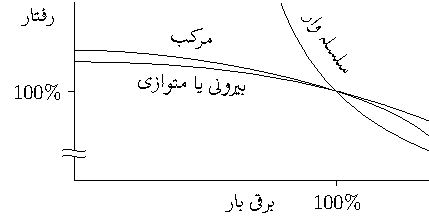
\includegraphics{figDCmotorSpeedVersusLoad}
\caption{یک سمتی موٹر کی میکانی بوجھ بمقابلہ رفتار کے خط۔}
\label{شکل_یکسمتی_موٹر_رفتار_بالمقابل_بار}
\end{figure}

متوازی جڑی یا بیرونی ہیجان موٹر تقریباً معین رفتار ہی برقرار رکھتی ہے۔اس کی رفتار بے بوجھ حالت سے پوری طرح بوجھ بردار حالت تک تقریباً صرف پانچ فی صد گھٹتی ہے۔ان موٹروں کی رفتار نہایت آسانی سے میدانی لچھے کی برقی رو تبدیل کر کے تبدیل کی جاتی ہے۔ایسا میدانی لچھے کے ساتھ سلسلہ وار جڑی مزاحمت کی تبدیلی سے کیا جاتا ہے۔ان کی رفتار یوں وسیع حدوں کے مابین تبدیل کرنا ممکن ہوتا ہے۔موٹر پر لاگو بیرونی برقی دباؤ تبدیل کر کے بھی رفتار قابو کی جا سکتی ہے۔ایسا عموماً قوی الیکٹرانکس کی مدد سے کیا جاتا ہے۔

ان موٹر کی ساکن حال سے چالو کرتے لمحہ کی قوت گردشہ اور ان کی زیادہ سے زیادہ قوت گردشہ قوی لچھے تک برقی رو پہنچانے کی صلاحیت پر منحصر ہے یعنی یہ میکانی سمت کار پر منحصر ہے۔

سلسلہ وار جڑی موٹر پر لدی میکانی بوجھ بڑھانے سے اس کے قوی اور میدانی لچھوں میں برقی رو بڑھے گی۔ میدانی مقناطیسی بہاو بڑھے گی اور مساوات \حوالہ{مساوات_یکسمتی_دباؤ_رو_قوی_سلسلہ_وار}  کے تحت \عددیء{E_q} کم ہو گی جو موٹر کی رفتار کم ہونے سے ہوتی ہے۔ بوجھ بڑھانے سے ان موٹر کی رفتار کافی زیادہ کم ہوتی ہے۔ایسے موٹر ان جگہوں بہتر ثابت ہوتے ہیں جہاں زیادہ قوت گردشہ درکار ہو۔بڑھتی قوت گردشہ کے ساتھ ان کی رفتار کم ہونے سے ان کو درکار برقی طاقت قوت گردشہ کے ساتھ زیادہ تبدیل نہیں ہوتا۔

یہاں اس بات کا ذکر ضروری ہے کہ بے بوجھ سلسلہ وار جڑی موٹر کی رفتار خطرناک حد تک بڑھ سکتی ہے۔ایسے موٹر کو استعمال کرتے وقت اس بات کا خاص خیال رکھنا ضروری ہے کہ موٹر ہر لمحہ بوجھ بردار رہے۔

ساکن حالت سے موٹر چالو کرتے وقت   \عددیء{I_q} کی قیمت زیادہ ہوتی ہے جس سے زیادہ  مقناطیسی بہاو پیدا ہوتا ہے۔یوں چالو کرتے وقت موٹر کی قوت گردشہ خاصی زیادہ ہوتی ہے۔ یہ ایک اچھی خوبی ہے جس سے بوجھ بردار ساکن موٹر کو چالو کرنا آسان ہوتا ہے۔

مرکب موٹروں میں ان دو قسموں کی موٹروں کے خصوصیات پائے جاتے ہیں۔جہاں بوجھ بردار موٹر چالو کرنا ضروری ہو لیکن رفتار میں سلسلہ وار موٹر جتنی تبدیلی منظور نہ ہو وہاں مرکب موٹر کارآمد ثابت ہوتے ہیں۔

\ابتدا{مثال}
ایک \عددیء{75}  کلو واٹ \عددیء{415} وولٹ اور \عددیء{1200} چکر فی منٹ کی رفتار سے چلنے والے متوازی جڑی یک سمتی موٹر کے قوی لچھے کی مزاحمت \عددیء{0.072} اوہم اور اس کی میدانی لچھے کی مزاحمت  \عددیء{83.2} اوہم ہے۔موٹر جس بوجھ سے لدا ہے اس پر موٹر  \عددیء{1123} چکر فی منٹ کی رفتار سے چلتے ہوئے  \عددیء{112} ایمپیئر لے رہی ہے۔ 
\begin{itemize}
\item
میدانی برقی رو اور قوی لچھے کی برقی رو حاصل کریں۔
\item
موٹر کی اندرونی پیدا کردہ برقی دباؤ حاصل کریں۔
\item
اگر میدانی لچھے کی مزاحمت \عددیء{100.2} اوہم کر دی جائے  مگر قوی لچھے کی برقی رو تبدیل نہ ہو  تو موٹر کی رفتار حاصل کریں۔مرکز کی سیرابیت کو نظرانداز کریں۔
\end{itemize}

\begin{figure}
\centering
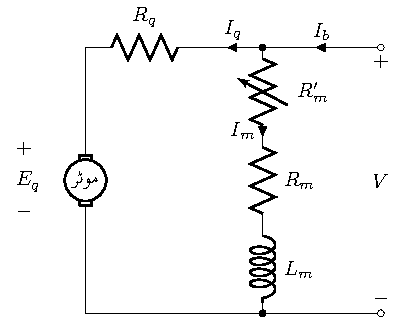
\includegraphics{figDCmotorExample}
\caption{یک سمتی موٹر کی مثال۔}
\label{شکل_یکسمتی_موٹر_کی_مثال}
\end{figure}

حل:
\begin{itemize}
\item
شکل \حوالہ{شکل_یکسمتی_موٹر_کی_مثال}  سے رجوع کریں۔\عددیء{415} وولٹ پر میدانی لچھے کی برقی رو
\begin{align*}
I_m=\tfrac{V}{R_m+R_m'}=\frac{415}{83.2}=\SI{4.988}{\ampere}
\end{align*}
ہو گی۔یوں قوی لچھے کی برقی رو \عددیء{I_q=I_b-I_m=112-4.988=\SI{107.012}{\ampere}} ہے۔
\item
یوں یک سمتی موٹر کی اندرونی پیدا کردہ برقی دباؤ
\begin{align*}
E_q=V-I_q R_q=415-107.012\times 0.072=\SI{407.295}{\volt}
\end{align*}
ہے۔
\item
اگر میدانی لچھے کی مزاحمت \عددیء{100.2} اوہم کر دی جائے  تب
\begin{align*}
I_m=\frac{V}{R_m+R_m'}=\frac{415}{100.2}=\SI{4.1417}{\ampere}
\end{align*}
ہو گی ۔
\item
اگر قوی لچھے کی برقی رو \عددیء{107.012} ایمپیئر ہی رکھی جائے تب 
\begin{align*}
E_q=V-I_q R_q=415-107.012 \times 0.072=\SI{407.295}{\volt}
\end{align*}
ہی رہے گی۔
\item
مساوات \حوالہ{مساوات_یکسمتی_پیدا_دباؤ_الف}  کی مدد سے  چونکہ اندرونی پیدا کردہ برقی دباؤ تبدیل نہیں ہوئی مگر مقناطیسی بہاو تبدیل ہوا ہے لہٰذا موٹر کی رفتار تبدیل ہو گی۔ان دو مقناطیسی بہاو اور رفتاروں پر اس مساوات کی نسبت
\begin{align*}
\frac{E_{q1}}{E_{q2}}=\frac{\frac{n}{2} \omega_1 N \phi_{m1}}{\frac{n}{2} \omega_2 N \phi_{m2}}
\end{align*}
میں چونکہ \عددیء{E_{q1}=E_{q2}} لہٰذا \عددیء{\omega_1 \phi_{m1}=\omega_2 \phi_{m2}} ہو گا۔مرکزی سیرابیت کو نظرانداز کرتے ہوئے چونکہ مقناطیسی بہاو میدانی دباؤ پر منحصر ہے جو از خود میدانی برقی رو پر منحصر ہے۔ لہٰذا اس آخری مساوات کو یوں لکھ سکتے ہیں۔
\begin{align*}
\frac{\omega_1}{\omega_2}=\frac{rpm_1}{rpm_2}=\frac{\phi_{m2}}{\phi_{m1}}=\frac{I_{m2}}{I_{m1}}
\end{align*}
جس سے نئی رفتار
\begin{align*}
rpm_2=\frac{I_{m1}}{I_{m2}} \times rpm_1=\frac{4.988}{4.1417} \times 1123=1352.47
\end{align*}
چکر فی منٹ حاصل ہوتی ہے۔اس مثال میں ہم دیکھتے ہیں کہ میدانی برقی رو کم کرنے سے موٹر کی رفتار بڑھتی ہے۔
\end{itemize}
\انتہا{مثال}
%
\ابتدا{مثال}
ایک \عددیء{60} کلو واٹ، \عددیء{415} وولٹ، \عددیء{1000} چکر فی منٹ متوازی جڑی یک سمتی موٹر کی قوی لچھے کی مزاحمت \عددیء{0.05} اوہم  اور میدانی لچھے کی \عددیء{60}  اوہم ہے۔بے بوجھ موٹر کی رفتار \عددیء{1000} چکر فی منٹ ہے۔میدانی لچھا \عددیء{1000} چکر کا ہے۔
\begin{itemize}
\item
جب یہ موٹر  ایمپیئر  لے رہی ہو اس وقت اس کی رفتار معلوم کریں۔
\item
\عددیء{140} ایمپیئر پر اس کی رفتار معلوم کرین۔
\item
\عددیء{210} ایمپیئر پر اس کی رفتار معلوم کرین۔
\item
اس موٹر کی رفتار بالمقابل قوت گردشہ گراف کریں  ۔
\end{itemize}

\begin{figure}
\centering
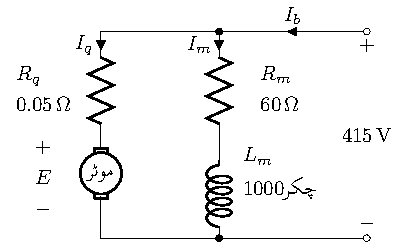
\includegraphics{figDCparallelMotorExample}
\caption{متوازی جڑی موٹر کی مثال۔}
\label{شکل_یکسمتی_متوازی_موٹر_کی_مثال}
\end{figure}

حل:
\begin{itemize}
\item
%
\begin{figure}
\centering
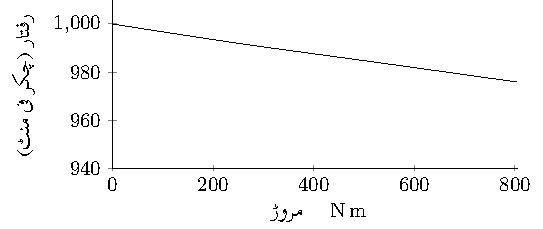
\includegraphics{figDCmotorSpeedVersusTorque}
\caption{رفتار بالمقابل قوت گردشہ۔}
\label{شکل_یکسمتی_رفتار_بالمقابل_مروڑ}
\end{figure}

شکل \حوالہ{شکل_یکسمتی_متوازی_موٹر_کی_مثال} میں یہ موٹر دکھائی گئی ہے۔متوازی میدانی لچھے کی برقی رو پر بوجھ لادنے سے کوئی فرق نہیں پڑتا۔لہٰذا میدانی مقناطیسی بہاو بے بوجھ اور بوجھ بردار موٹر میں یکساں ہے۔بے بار یک سمتی موٹر کی قوی لچھے کی برقی رو \عددیء{I_q}  قابلِ نظر انداز ہوتی ہے۔اس طرح مساوات \حوالہ{مساوات_یکسمتی_دباؤ_رو_قوی_سلسلہ_وار}  اور مساوات \حوالہ{مساوات_یکسمتی_چکر_بالمقابل_رفتار}  سے  
\begin{align*}
E_q&=V-I_q R_q=415-0\times R_q=\SI{415}{\volt}\\
I_m&=\frac{V}{R_m}=\frac{415}{60}=\SI{6.916}{\ampere}
\end{align*}
یعنی \عددیء{415} وولٹ محرکی برقی دباؤ پر رفتار \عددیء{1000} چکر فی منٹ یا \عددیء{16.66} چکر فی سیکنڈ ہے۔\عددیء{70} ایمپیئر برقی بوجھ پر بھی \عددیء{I_m=\SI{6.916}{\ampere}} ہی ہے جبکہ 
\begin{align*}
I_q=I_b-I_m=70-6.916=\SI{63.086}{\ampere}
\end{align*}
لہٰذا مساوات \حوالہ{مساوات_یکسمتی_دباؤ_رو_قوی_سلسلہ_وار}  سے اس صورت میں
\begin{align*}
E_q=V-I_q R_q=415-63.086 \times 0.05=\SI{411.8458}{\volt}
\end{align*}
اور مساوات \حوالہ{مساوات_یکسمتی_چکر_بالمقابل_رفتار}  سے رفتار (چکر فی منٹ) یوں حاصل ہوتا ہے
\begin{align*}
rpm=\frac{e_q}{e_{q0}} rpm_0=\frac{411.8458}{415} \times 1000=991.95
\end{align*}
%
\item
یہی کچھ دوبارہ کرتے ہیں۔یہاں \عددیء{I_b=\SI{140}{\ampere}} ہے۔
\begin{align*}
I_q&=I_b-I_m=140-6.916=\SI{133.084}{\ampere}\\
E_q&=415-133.084 \times 0.05=\SI{408.3458}{\volt}\\
rpm&=\frac{408.3458}{415} \times 1000=983.96
\end{align*}
%
\item
یہاں \عددیء{I_b=\SI{210}{\ampere}} ہے۔
\begin{align*}
I_q&=I_b-I_m=210-6.916=\SI{203.084}{\ampere}\\
E_q&=415-203.084 \times 0.05=\SI{404.8458}{\volt}\\
rpm&=\frac{404.8458}{415} \times 1000=975.83
\end{align*}
%
\item
موٹر میں طاقت کے ضیاع کو نظر انداز کرتے ہیں۔ یوں اس کی میکانی طاقت اسے فراہم کی گئی برقی طاقت کے برابر ہو گی یعنی
\begin{align}
e_q I_q=T \omega
\end{align}
یوں پچھلے جزوسے حاصل جوابات کی مدد سے بے بوجھ موٹر کی قوت گردشہ  صفر ہو گی یعنی \عددیء{T_0=\SI{0}{\newton \meter}}  جبکہ \عددیء{70}  ایمپیئر پر قوت گردشہ کی قیمت
\begin{align*}
T_{70}=\frac{e_q I_q}{\omega}=\frac{411.8458 \times 63.086}{2 \times \pi \times 16.5325}=\SI{250}{\newton \meter}
\end{align*}
ہو گی۔یہاں \عددیء{991.95} چکر فی منٹ کی رفتار کو \عددیء{16.5325} ہرٹز لکھا گیا ہے۔ اسی طرح
\begin{align*}
T_{140}&=\frac{e_q I_q}{\omega}=\frac{408.3458 \times 133.084}{2 \times \pi \times 16.399}=\SI{527}{\newton \meter}\\
T_{210}&=\frac{e_q I_q}{\omega}=\frac{404.8458 \times  203.084}{2 \times \pi \times 16.26}=\SI{805}{\newton \meter}
\end{align*}
یہ نتائج شکل \حوالہ{شکل_یکسمتی_رفتار_بالمقابل_مروڑ}  میں گراف کئے گئے ہیں۔
\end{itemize}

\انتہا{مثال}
